54. \begin{figure}[ht!]
\center{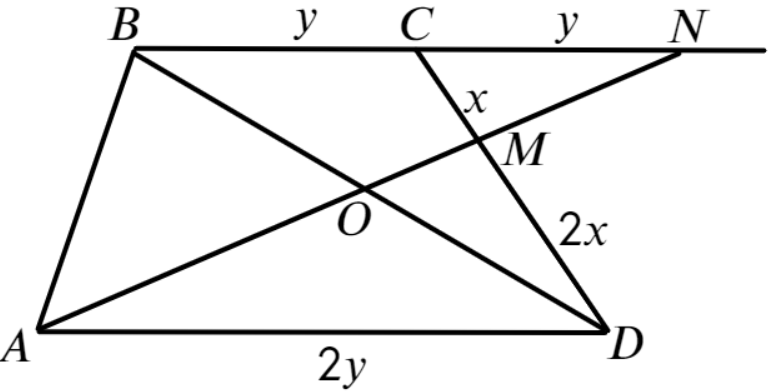
\includegraphics[scale=0.35]{g9-54.png}}
\end{figure}\\
Обозначим $CM=x,\ DM=2x,\ BC=y,\ AD=2y.$ Продлим $AM$ до пересечения с продолжением $BC$ в точке $N.$ Треугольники $CMN$ и $AMD$ подобны по двум углам (накрест лежащие  $MCN$ с $MDA$ и $MNC$ с $MAD$, значит $\cfrac{CN}{AD}=\cfrac{CM}{DM}=\cfrac{1}{2},\ CN=y.$ Тогда $BN=y+y=2y=AD$ и треугольники $OBN$ и $ODA$ равны по стороне и двум прилежащим к ней углам (накрест лежащие $OBN$ с $ODA$ и $ONB$ с $OAD),$ поэтому $BO=OD$ и $BO:OD=1:1,$ а также $AO=ON.$ Из подобия треугольников $CMN$ и $AMD$ получаем $AM=2MN.$ Значит, $MN=\cfrac{1}{3}AN,$ а $AO=\cfrac{1}{2}AN,$ поэтому $OM=AN-AO-MN=\cfrac{1}{6}AN.$ Таким образом, $AO:OM=\cfrac{1}{2}AN:\cfrac{1}{6}AN=3:1.$\\
